% load the document class KOMA-Script Report
\documentclass[	
		a4paper,			% Papierformat waehlen
		11pt,				% Schriftgroesse
%		draft,				% Randueberschreitungen werden schwarz markiert
%		DIV13,				% Unterteilung des Blatts in DIVxx - xx Teile              OBSOLETE
						% Je kleiner die Zahl umso groesser die Raender
						% Um Optimale Anpassung zu erhalten : DIVcalc + \typearea...
%		BCOR5mm,			% Bindekorrektur BCORXmm - Xmm breit                       OBSOLETE
		%pointlessnumbers,		% KEIN ZWEITER PUNKT IN DER NUMMERIERUNG DER ÜBERSCHRIFTET 2.2 statt 2.2.	
%
%      KOPF/FUSSZEILE
%		headinclude,			% Head gehoert mit zum Textblock/auskommentiert im Seitenrand
		headsepline,			% Trennlinie zwischen Kopf und Text, schaltet automatisch 
						% headinclude mit ein
%		footinclude,			% wie Head nur Foot
%		footsepline,			% wie headsepline
%
%      LAYOUTPARAMETER
%		twocolumn,			% Zweispaltige Texte
		onecolumn,			% Einspaltig
%		twoside,			% Zweiseitiger Druck re -li sind gespiegelt vom Satzspiegel
		oneside,			% Einseitig
%		openright,			% Sollte bei zweiseitigem Druck eignestellt werden
%		cleardoublestandard		% Alles fuer 2Seitige mit openright: Kolumnentitel linke Seite
%		cleardoubleplain		% nur Seitenzahlen linke Seite
%		cleardoubleempty		% linke Seite ganz leer
%		chapterprefix,			% Kapitel wir zu beginn eines Kapitels ausgegeben
%		appendixprefix,			% Anhang wird vor Kapiteln im Anhang ausgegeben
		headings=normal,		% kleine ueberschriften, oder small-, oder big-headings.
						% Standard ist Big
%
%	TABELLENEIGENSCHAFTEN
		captions=tableheading,		% Um richtigen Abstand fuer Ueberschrift zu erhalten, 
						% Ueberschrift wird genommen
%
%	VERZEICHNISEINSTELLUNGEN
%		tocleft,			% Setzt das Inhaltverzeichnis nicht eingerueckt nach links
%		liststotoc,			% Abb.- und Tab.Verzeichnisse ins Inhaltsverzeichnis
%		liststotocnumbered, 		% wie liststotoc nur mit Gliederungspunktangabe
%		bibtotoc,			% Literaturverzeichnis ins Inhaltverzeichnis
%		bibtotocnumbered,		% s.o. nur mit Gliederungsebene
%		idxtotoc,			% Eintrag ins Inhaltsverzeichnis fue Index
%		openbib,			% Veraendert aussehen des Lit.-Verzeichnisses
%	Language
%		ngerman,			% to pass as standard to all packages
]{scrreprt}

% load packages for european, espacially german users

\usepackage[T1]{fontenc}			% Schriften fuer Europaeische Zeichen passend Kodiert
\usepackage[utf8]{inputenc}        		% Eingabe von Umlauten, ss usw. - 
						% utf8: kann nicht jeder Editor speicher, aber plattformuebergreifend
						% latin1: Unix, VMS, Windows
						% ansinew: Windows
						% latin9: wie latin1, jedoch mit Eurozeichen
						
\usepackage[					% Passt Konventionen an Sprache an
	     english, 
	     ngerman				% ngerman: Neue Deutsche Rechtschreibung
	    ]{babel}				% z.B. UKenglish, USenglish, canadian, german, austrian, naustrian
	    
%\hyphenation{}					% Trennung von Woertern falls nicht automatisch korrekt erkannt
%\usepackage{icomma}				% Bei deutscher Schreibweise, damit keine

%\usepackage[scaled=0.66]{luximono}		% Schrift fuer Typewriter - Quellcode ~8pt
				

% Fuer optimale Anpassung des Satzspiegels
%\typearea[current]{calc}			% Bestimmt Rasterzahl aus Schriftgroesse und Anzahl der 		
						% Zeichen/Woerter pro Zeile

% FUSS UND KOPFZEILENANPASSUNG
%\pagestyle{plain}				% empty: Keine Kopf/Fusszeile
						% plain: Seitenzahl am Fussende
						% headings: aktiviert lebende Kolumnentitel (Kapitel im Kopf)
						% myheadings : eigene Kopf- fußzeilen
						% fancy: Erlaubt die Verwendung der in dem Paket "fancyhdr" 
						% definierten Befehle zur Erstellung eigener Kopf- und Fußzeilen

%%error
% scrpage2 ist obsolete!
%\usepackage[
%	    automark				% takes the chapter variant
%	   ]{scrpage2}				% Fuer eigene Kopf/Fusszeilen, ermoeglicht. 
% stattdessen scrlayer-scrpage:

\usepackage{scrlayer-scrpage}
\pagestyle{scrheadings} %, scrplain}
\clearscrheadings				% clear old header style
\clearscrplain					% clear plain header style
\clearscrheadfoot				% clear foot style
%\automark[section]{chapter}
\automark[chapter]{chapter}
\ohead{\pagemark}				% beide Außenseiten des Headers --Seitenzahl
\ihead{\headmark}				% beide Innenseiten Headers -- Chapter
%\chead						% zentriert 
%\lehead					% left even
%\cehead
%\rehead
%\lohead					% left odd
%\cohead
%\rohead
%%


%\lehead{\leftmark}
%\lohead{\rightmark}
%\ofoot[\pagemark]{}				% auf plain seiten Seitenzahl außen
									
% Schriftfamilien Laden
\usepackage{lmodern}				% Laedt die Schriftart Latin-Modern fuer Text
%\usepackage{courier}
%\rmfamily
%\sffamily
%\ttfamily
%\renewcommand{\rmdefault}{
%			  pbk	% Bookman
%			  phv	% Helvetica
%			  cmr	% CM Roman
%			  ppl	% Palatino
%			  ptm	% Times Roman
%			  pag	% Avant Garde
%			  pcz	% Zapf Chancery
%			 }
%\renewcommand{\familydefault}{\sfdefault}

% Alternativ Schriftart (Textshchrift) ändern über usepackage:
\usepackage{
%	    mathpazo	% Palatino
%	    mathptmx	% Times
%	    avant	% Avant Garde
%	    courier	% Courier
%	    chancery	% Zapf Chancery
	    bookman	% Bookman
%	    newcent	% New Century Schoolbook
%	    charter	% Charter
%	    helvet	% Helvetica
} 
%\usepackage[scaled=0.92]{helvet}		% Helvetica, ist größer als Times und sollte bei verwendung beider skaliert werden.

% Im Dokument wechslen:
%\fontfamily{pbk}\selectfont

\usepackage[
	    babel,
%	    german=guillemets,  		% franz. <<  >>
	    german= quotes,			% deutsche Anfuehrungszeichen "
	   ]{csquotes}				% Laden der richtigen Anfuehrungszeicehn fuer deutsche sprache
						% = quotes fuer englische sprache



	   
%\usepackage{setspace}				% Fuer Abstaende im Dokument
%\onehalfspacing				% aendert Zeilenabstand auf 1 1/2
									
%\usepackage{microtype}				% optischer Randausgleich in PDF's
									% ungeeignet fuer internettexte o.ae.	
	   
%\usepackage[					% Papierformate auf denen gedruckt werden soll
%		a0,b0,
%		a1,b1,
%		a2,b2,
%		a3,b3,
%		a4,b4,
%		a5,b5,
%		a6,b6,
%		letter,
%		legal,
%		executive,
%		center,				% zentrierter druck
%		landscape,			% querformat
%		]{crop}
	 
									
\usepackage[a4paper]{geometry}			% Anpassung von Seitenraender per Hand
\geometry{					% Wenn Zweiseitig-> left->inner : right->outer	
	    top=2cm, 				% Weitere Moeglichkeiten: height - Texthoehe, width - Textbreite
	    bottom=5cm,
	    inner=2cm,
	    outer=3cm
         }	

\setlength{\headheight}{1.5cm}
\setlength{\voffset}{0.5cm}


\usepackage[					% To set Text at a specific 
		absolute,			% absolute - absolute position on the page
		overlay,			% overlay - if using absolute option text is placed below other things
%		showboxes,			% showboxes - shows boxes around the text
%		noshowtext,			% noshowtext - just show the box if it is on
%		verbose,			% verbose - package writing things to output like calculations
%		quiet,				% quiet turns this off : verbose = default
	    ]{textpos}

\usepackage[
	    hyperref 	= false,		% switch off hyperref hack
	    float 	= true,			% switch off float hack
	    listings 	= true,  		% switch off listings hack
	   ]{scrhack}				% to get rid off the warning @addtocbasic

	   
%\usepackage{anyfontsize} % hilft gegen font shape not available, was wegen \DeclareMathSizes auftreten kann
\usepackage{relsize}                            % für größere und kleinere Gleichungen über den Befehl \mathlarger bzw. \mathsmaller, auch \textlarger und \textsmaller

\usepackage{lscape}

\usepackage{color}				% to use colors, espacially for source codes
\usepackage[%
%	    table				% Zum automatischen Laden des Pakets colortbl - fuer Tabellen
	   ]{xcolor}				% for Hyperref package, that one can say red than rgb values

	   
	   
\definecolor{mygreen}{rgb}{0,0.6,0}
\definecolor{forestgreen}{rgb}{0.0, 0.27, 0.13}
\definecolor{mygray}{rgb}{0.5,0.5,0.5}
\definecolor{mymauve}{rgb}{0.58,0,0.82}
\definecolor{lila}{rgb}{0.6, 0.4, 0.8}
\definecolor{lavendel}{rgb}{0.75, 0.58, 0.89}
\definecolor{applegreen}{rgb}{0.55, 0.71, 0.0}
\definecolor{azure}{rgb}{0.0, 0.5, 1.0}
\definecolor{yellow}{rgb}{0.99, 0.93, 0.0}
\definecolor{brown}{rgb}{0.59, 0.29, 0.0}
\definecolor{cinnamon}{rgb}{0.82, 0.41, 0.12}
\definecolor{pumpkin}{rgb}{1.0, 0.46, 0.09}
\definecolor{pink}{rgb}{0.91, 0.25, 0.78}

\definecolor{DOGGYbg}{RGB}{80,90,100} %HAW Color
\definecolor{DOGGY}{RGB}{26,60,116} % HAW Color 2
\definecolor{lgray}{RGB}{240,240,240} %HAW Color
\definecolor{darkgreen}{RGB}{50,150,50} %HAW Color

\definecolor{brightgray}{RGB}{230,230,230}

\newcommand{\boxColorForOne}{black}
\newcommand{\boxColorForZero}{lightgray}
\newcommand{\boxColorForSqrt}{green}

\newcommand{\textColorForOne}{white}
\newcommand{\textColorForZero}{black}
\newcommand{\textColorForSqrt}{black}

\newcommand{\boxHeightL}{11}
\newcommand{\boxWidthL}{11}
\newcommand{\boxHeightS}{11}
\newcommand{\boxWidthS}{11}
\newcommand{\boxWidthWide}{13}
\newcommand{\boxHeightHigh}{13}



\newcommand{\myboxOnePos}{\colorbox{\boxColorForOne}{\makebox(\boxWidthL,\boxHeightL){\textcolor{\textColorForOne}{}}}}
\newcommand{\myboxOneNeg}{\colorbox{\boxColorForOne }{\makebox(\boxWidthL,\boxHeightL){\textcolor{\textColorForOne}{-}}}}
\newcommand{\myboxZero}  {\colorbox{\boxColorForZero}{\makebox(\boxWidthL,\boxHeightL){\textcolor{\textColorForZero}{}}}}
\newcommand{\myboxSqrtPos}{\colorbox{\boxColorForSqrt}{\makebox(\boxWidthL,\boxHeightL){\textcolor{\textColorForSqrt}{}}}}
\newcommand{\myboxSqrtNeg}{\colorbox{\boxColorForSqrt}{\makebox(\boxWidthL,\boxHeightL){\textcolor{\textColorForSqrt}{-}}}}

\newcommand{\myBlackBox}{\colorbox{black}{\makebox(\boxWidthS,\boxHeightS){\textcolor{\textColorForSqrt}{}}}}
\newcommand{\myGrayBox}{\colorbox{gray}{\makebox(\boxWidthS,\boxHeightS){\textcolor{\textColorForSqrt}{}}}}
\newcommand{\myLightgrayBox}{\colorbox{lightgray}{\makebox(\boxWidthS,\boxHeightS){\textcolor{\textColorForSqrt}{}}}}
\newcommand{\myDarkgrayBox}{\colorbox{darkgray}{\makebox(\boxWidthS,\boxHeightS){\textcolor{\textColorForSqrt}{}}}}

\newcommand{\myBlackBoxHigh}{\colorbox{black}{\makebox(\boxWidthS,\boxHeightHigh){\textcolor{\textColorForSqrt}{}}}}
\newcommand{\myBlackBoxWide}{\colorbox{black}{\makebox(\boxWidthWide,\boxHeightS){\textcolor{\textColorForSqrt}{}}}}
\newcommand{\myLightgrayBoxHigh}{\colorbox{lightgray}{\makebox(\boxWidthS,\boxHeightHigh){\textcolor{\textColorForSqrt}{}}}}
\newcommand{\myLightgrayBoxWide}{\colorbox{lightgray}{\makebox(\boxWidthWide,\boxHeightS){\textcolor{\textColorForSqrt}{}}}}

\usepackage{tcolorbox} 

\newtcolorbox{mytextbox}[1]{%
    tikznode boxed title,
    enhanced,
    arc=0mm,
    interior style={white},
    attach boxed title to top left= {xshift=0.5cm, yshift=-\tcboxedtitleheight/2},
    fonttitle=\bfseries,
    colbacktitle=white,coltitle=black,
    boxed title style={size=normal,colframe=gray,boxrule=0pt},
    title={#1}}
\usepackage[%
%	    leqno,				% Nummern linksbuendig
%	    reqno,				% Nummern rechtsbuendig (Standard)
%	    fleqn,				% Gleichungen linksbuendig statt zentriert
	   ]{amsmath}
\usepackage{amsfonts}				% Um Zahlenraeume richtig darzustellen
\usepackage{mathtools}


% Betragsstriche über \abs, Doppelbetragsstriche über \norm
\DeclarePairedDelimiter\abs{\lvert}{\rvert}%
\DeclarePairedDelimiter\norm{\lVert}{\rVert}%

\usepackage[%
	    thinlines,				% dünne linien
%	    thicklines,				% dicke linien
	   ]{easybmat}				% For Matrices with dottet lines between fields, horizontal or vertical
%\usepackage{MnSymbol}				% Zusaetzliche Zeichen
\usepackage{trsym}				% Fuer Laplace-Fourier-Symbole
\usepackage{mathrsfs}				% Fuer Matheschrift
\usepackage{xfrac}
\usepackage{nicefrac}
\usepackage{esint}
%\usepackage{exscale} % lässt Klammern in Gleichungen verschwinden!!
%\DeclareMathSizes{10.95}{30}{15}{15} % 10.95 für 11pt in documentclass

\def\mathunderline#1#2{\color{#1}\underline{{\color{black}#2}}\color{black}}

\usepackage{soul}
\usepackage{graphicx} 				% für Grafik-Einbindung
\usepackage{subfigure}				% Für Untergrafiken, wenn eine eigene Bildunterschrift erwuenscht
\usepackage[hypcap=false]{caption}				% für Captions bei Grafiken ohne figure Umgebung wie in Minipage nötig
\usepackage[%
	    update				% if pdf conversion is older than eps file, new conversion is done
	   ]{epstopdf}				% eps to pdf needs for pdflatex - after graphicx

	   


\usepackage{tikz}
%\usepackage{background}
\usetikzlibrary{thedecorations, arrows,shapes, automata, positioning, calc, backgrounds, decorations.pathreplacing,decorations.pathmorphing, matrix}


\newcommand{\tikzmark}[1]{\tikz[overlay, remember picture] \coordinate (#1);}

\tikzset{node/.style={draw,shape=circle}}
\newcommand{\order}[2][th]{\ensuremath{{#2}^{\mathrm{#1}}}}
\usepackage{multirow}				% Fuer Mehrzeilige Zellen
\usepackage{multicol}
%\usepackage{array}					% Festlegen von Breiten, Präfixe, Suffixe
% see also package siunitx - damit Spalten mit Zahlen auf bestimmte Länge ausgerichtet werden
\usepackage{tabularx}				% Zum festlegen der Gesamtbreite der Tabelle & verwenden von X fuer 
									% variable Spaltenbreite
%\usepackage{longtable}				% Tabelle ueber mehr als eine Seite
\usepackage{ltxtable}				% longtable + tabularx eigenschaften

%\usepackage{rotating}				% Querformat der Tabelle
									% !!! Vorsicht !!!
									% tablecaptionabove wird nicht ausgewertet,
									% Einfuegen von \vskip\abovecaptionskip --> Nur unter KOMA Script
%\usepackage{ctable}					% For tables with footnote under the table directly


\setlength{\arraycolsep}{0.4pt}
\delimitershortfall=0pt % Höhereduzierung der Klammern von Matrizen gegenüber dem Inhalt

\usepackage{tabu} % fuer farbige Zeilen in Tabellen
\usepackage[  % Packet ist jetzt glossaries-extra statt glossaries - keine Ahnung, ob die es die auskommentierten Optionen gibt!
	    xindy,%={language=german-modern, codepage=utf8},
	    automake,				
	    numberedsection,
%	    toc,      				% Fügt Eintrag ins Inhaltsverzeichnis hinzu, defualt false
	    nonumberlist,			% keine Ausgabe der Seitenzahlen
%	    nowarn,				% unterdrückt alle warungen des pakets
%	    nomain,				% kein hauptglossary wird erzeugt, acronym oder newglossary um Einträge zu erzeugen
%	    sanitize={%				% unterdrückt die keys für einträge oder fügt sie hinzu
%	    name        = false,%
%	    description = false,%
%	    symbol      = false},%
%	    translate = true,			% zur übersetzung von einträgen - siehe doku, default false
	    hyperfirst = true,			% erzeugt hyperlink zum glossar bei erster verwendung, default true
%	    hyper = false,			% Hyperlinks ausschalten
%	    numberline,				% Eintrag ins toc mit Nummerierung
%	    section=section,			% in welcher ebene der eintrag, default chapter if loaded sonst section
%	    style = long,			% default list, sonst: long, super, tree
%	    nolong,				% pakete für longtable werden nicht geladen und befehle nicht definiert
%	    nosuper,				% supertabular wird nicht geladen, pakete nicht definiert
%	    nolist,				% list wird nicht geladen definiert
%	    notree,				% gloassrytree wird nicht geladen definiert
%	    nostyles,				% keine styles werden geladen, eigene definieren
%	    counter = page,			% page default, or any other counter
%	    sort = def,				% def - sortiert nach definition, standard(default)-sortiert nach sort key, sonst name, use - sortieren nach reihenfolge wie sie im dokument vorkommen
%	Acronym options
%	    acronym,  				% Seperate Liste für Acronyme zum Glossary, default - false
%	    acronymlist={},			% wenn mehr als eine abkürzungsliste, muss diese hier mit angegeben werden damit das glossary als acronym behandelt wird
%	    description,			% erlaubt eine zusätzliche beschreibung
%	    footnote,				% schreibt die long version als fußnote bei erster nutzung
%	    smallcaps,				% acronyme werden als kapitelchen angezeigt
%	    smaller,				% kleinere schrift, laden von relsize für befehl textsmaller erforderlich
%	    dua,				% langform wird immer ausgegeben
	    shortcuts,				% um selbe befehle wie acronym paket zu haben
	   ]{glossaries-extra}		


\GlsSetXdyCodePage{duden-utf8}

% sorgt dafür, dass die Erklärungen alle gleich eingerückt sind
\setglossarystyle{long}
\renewcommand{\glsnamefont}[1]{\textbf{#1}}

% Bachlorarbeit.gls erzeugen:
% $ cd Bachelorarbeit
% $ makeglossaries "Bachelorarbeit"

\makeglossaries 

\newabbreviation{1d-dft}{1D-DFT}{Eindimensionale Diskrete Fouriertransformation}
\newabbreviation{2d-dft}{2D-DFT}{Zweidimensionale Diskrete Fouriertransformation}

\newabbreviation{adc}{ADC}{Analog Digital Converter}
\newabbreviation{adu}{ADU}{Analog Digital Umsetzer}
\newabbreviation{amr}{AMR}{anisotroper magnetoresistiver Effekt}
\newabbreviation{amr2}{AMR}{anisotropen magnetoresistiven Effekt}
\newabbreviation{asic}{ASIC}{Application Specific Integrated Circuit, \textit{dt.: Anwendungsspezifischer Integrierter Schaltkreis}}

\newabbreviation{dac}{ADC}{Digital Analog Converter}
\newabbreviation{dau}{ADU}{Digital Analog Umsetzer}
\newabbreviation{dct}{DCT}{Diskrete Cosinus Transformation}
\newabbreviation{dft}{DFT}{Diskrete Fouriertransformation}

\newabbreviation{idft}{IDFT}{Inverse Diskrete Fouriertransformation}
\newabbreviation{isar}{ISAR}{Integrated Sensor Array}

\newabbreviation{ft}{FT}{Fouriertransformation}
\newabbreviation{fft}{FFT}{Fast Fouriertransformation}

\newabbreviation{lsb}{LSB}{Least Significant Bit}

\newabbreviation{msb}{MSB}{Most Significant Bit}

\newabbreviation{tmr}{TMR}{tunnelmagnetoresistiver Effekt}
\newabbreviation{tmr2}{TMR}{tunnelmagnetoresistiven Effekt}



\glsaddall

\setlength\LTleft{0pt}
\setlength\LTright{0pt}
\setlength\glsdescwidth{0.8\hsize}


% Hyperref for PDFLATEX with links    
\usepackage[
	    draft 	= false,			% all hypertext options are turned off
	    final 	= true, 			% all hypertext options are turned on
	    raiselinks 	= true,				% Allow links to reflect real height - e.g. with pictures
	    breaklinks	= false,			% false=Do not break a line within a link
	    backref	= false,			% false=no backlinks in the bibliography
	    pagebackref = false,			% false=no pagebacklinks in bibliography
%	    linktocpage = true,				% true=makes page-no linked and not text in TOC,LOF and LOT
	    linktoc	= all,
%			  none,
%			  section,
%			  page,
	    colorlinks	= false,			% true=Colors the text of links and anchors
%	    linkcolor 	= red, 				% Color for normal internal links.
%	    anchorcolor = black, 			% Color for anchor text.
%	    citecolor 	= green, 			% Color for bibliographical citations in text.
%	    filecolor 	= cyan, 			% Color for URLs which open local files.
%	    menucolor 	= red,				% Color for Acrobat menu items.
%	    runcolor 	= filecolor,			% Color for run links (launch annotations).
%	    allcolors 	= red,				% Set all color options (without border and field options).
	    urlcolor 	= blue,				% Color for linked URLs.
%	    allbordercolors  =red,			% Set all colors
%	    citebordercolor =green,			% cite color
%	    filebordercolor =cyan,			% file color
%	    linkbordercolor =red,			% link color
%	    urlbordercolor  =blue,			% url color
%	    pdfborder = 0 0 0,				% weder farbige links noch umrandung			
%	    menubordercolor =red,			% set menu color
%	    frenchlinks = 	false,			% Use small caps instead of color for links.
	    bookmarks	=	true,			% true=Bookmarks are added to the pdf
	    bookmarksopen=	false,			% false=Bookmarks not open when opening the pdf
	    bookmarksnumbered=true,			% true= Eintraege sind nummeriert
%	    pdfpagemode	=	FullScreen,		% File is opened in Full Screen
%	    pdfstartview=	fit,			% Fit size when opening pdf
	    pdfpagelabels=	true,			% true = Roemische Zahlen usw werden dargestellt,
							% false= fortlaufende nummerierung
	   ]{hyperref}
\hypersetup{hidelinks}

\input{preamble/listings.tex}
\usepackage[
	    official,
	    right				% Position of the Euro-Sign. verwendung: \euro oder \EUR{123,45}
	   ]{eurosym}


% Loading unit options                



\usepackage[Algorithmus]{algorithm} 			% deutsche notation im titel

% Zitate die in den Referenzen aufscheinen, aber nicht unbedingt im Text zitiert werden m�ssen
% Literatur, die mit \nocite oder \cite zitiert wird, mu� im .bib File erfasst werden!
\nocite{Guenther:2002}
\nocite{Lamport:1995}
\nocite{Goossens:2000}
\nocite{Kohm:2003}
\nocite{Hunt:2003}
\nocite{Boehm:2002}
\nocite{Schmatz:2004}
\nocite{Streitz:2005}
\nocite{HP:2004}
\nocite{Luede:2004}
\nocite{Demarco:1999}
\nocite{Kollakowski:2004}
\nocite{Dawson:2003}
\nocite{Poenicke:1988}
\nocite{Kruse:2000}
\nocite{Nilsson:1998}
\nocite{Heinsohn:1999}
\nocite{Luger:2001}
\nocite{Kuehnel:2001}
\nocite{Bigus:2001}
\nocite{Ferber:2001}
\nocite{Wooldridge:2002}
\nocite{KuroseRoss:2002}
\nocite{Vogt:2001}
\nocite{Roetzer:1999}
\nocite{P3P:2004}
\nocite{CPEX:2004}
\nocite{Duden:1997}
\nocite{Hoerauf:2001}
\nocite{Schirru:2004}
\nocite{Babic:2003}
\nocite{Luepke:2004}

	
\usepackage{bbding}					% to get cross and check symbol

\usepackage{enumerate}					% schicke Nummerierung

\usepackage{pdfpages}					% Zum Laden und einbinden von PDF-Seiten
\usepackage{pgfpages}
\usepackage{float}					% für floats (figures) in einer Minipage (geht nicht!!)
\usepackage{booktabs}					% Fuer besseres aussehen der Linien
\usepackage{framed}					% for use of newtheorem with a coloured box

\usepackage{titling}
\author{Thomas Lattmann}
\title{Chipimplementation einer zweidimensionalen Fouriertransformation für die Auswertung eines Sensor-Arrays}
\date{23.4.2018}
			
% INDEX ERZEUGEN - falls gewuenscht muessen beide direkt so eingebunden werden
%\usepackage{index}
%\makeindex

%\makenomenclature					% damit Symbolverzeichnis erzeugt wird

% Symbolverzeichnis erzeugen - lade dazu mit %%%%%%%%%%%%%%%%%%%%%%%%%%%%%%%%%%%%%%%%%%%%%%%%%%%%%%%%%%%%%%%%%%%%%%%%%%%%%%%
%  Author     : Dennis Schuethe        Date    : 28.12.2011                   %
%  Filename   : symbolpage.tex         Version : 1.0                          %
%  Information: This file will create the nomenclature and should be designed %
%               the way you want to. There are two options:                   %
%               1. Use the normal nomenclature which is given and created by  %
%                  the nomencl.sty -> see package declarations                %
%               2. To have more than one column for the nomenclature, then    %
%                  use the \begin{multicols}, but this cause a bad look,      %
%                  because the name is printed within the columns, better use %
%                  option 3                                                   %
%               3. Find the nomencl.sty and then rewrite the lines 160 and    %
%                  164 as it is shown below, then you need to add the         %
%                  \chapter*{\nomname} or \section*{\nomname} by yourself     %
%-----------------------------------------------------------------------------%
%  Changelog  :                                                               %
%  28.12.2011  opened this file                                               %
%              may the nomencl.sty could be changed by adding this as option, %
%              need to try a workaround                                       %
%  %
%%%%%%%%%%%%%%%%%%%%%%%%%%%%%%%%%%%%%%%%%%%%%%%%%%%%%%%%%%%%%%%%%%%%%%%%%%%%%%%


%157 \def\thenomenclature{%
%158  \@ifundefined{chapter}%
%159  {
%160    %\section*{\nomname}
%161    \if@intoc\addcontentsline{toc}{section}{\nomname}\fi%
%162  }%
%163  {
%164    %\chapter*{\nomname}
%165    \if@intoc\addcontentsline{toc}{chapter}{\nomname}\fi%
%166  }%

%\renewcommand{\nomname}{newname}	% New name for the nomenclature
%\chapter*{\nomname}				% Do the heading for this chapter(section)
% else			
% newpage							% only if chapter command is not used
%\begin{multicols}{2}				% Do multiple columns - use package multicol
\printnomenclature %[2cm] 			% Symbolverzeichnis mit breite xcm für symbole, std is 1cm
%\end{multicols} das Verzeichnis 
%\usepackage[
%	     intoc,					% Eintrag des Abkuerzungsverzeichnis
%	     notintoc,					% Kein Eintrag - default
%	     english,					% Ueberschrift in English (default)
%      	     german,					% in deutsch
%	    ]{nomencl}


% Loading label options               
\usepackage[ngerman]{varioref}		            	% To get automatic "see Section xy on page xx"
%\usepackage[german]{fancyref}		    		% same as varioref, except this is setting section automatically
							% Options in []-brackets:
							% language, e.g. english, ngerman - last entry is main-language
							% paren - sets the reference in ()-brackets
							% plain - no pagenumber in the reference
							% -----------------------------------------
							% standard prefixes used by fancyref:
							% sec, chap, part, fig, tab, enum, eq, fn
%\fancyrefchangeprefix{\fancyrefchaplabelprefix}{cha} 	% sets a new prefix for the label chap




% Pseudocode 			 %
\usepackage[noend]{algpseudocode}


\title[Implementierung der 1D-DFT in VHDL und Erweiterung zur 2D-DFT, Aktueller Stand der BA]{\textbf{Implementierung der 1D-DFT in VHDL\\ und Erweiterung zur 2D-DFT}\\ \vspace{1cm} Aktueller Stand der Bachelorarbeit}
\vspace{1cm}
\author[TL]{Thomas Lattmann}
\date[8.1.2018]{8.1.2018} 
\institute[HAW]{HAW-Hamburg, ISAR-Projektmeeting}


\begin{document}




% Define a background image for the first page
%\usebackgroundtemplate{\includegraphics[]{backT.pdf}}
%\usebackgroundtemplate{}

\usebackgroundtemplate{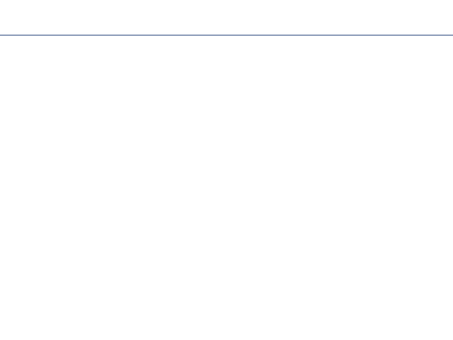
\includegraphics[scale=1]{img/back.pdf}}
%=============================================================================
	%\begin{frame}\frametitle{Inhalt}
	%	\tableofcontents
	%\end{frame}	
%=============================================================================

\frame{\titlepage}

\begin{frame}[t]\frametitle{Veranschaulichung}

\begin{minipage}{0.55\textwidth}
\begingroup
 \renewcommand*{\arraystretch}{0.8} % Zeilenabstand der Tabelle  
   $\Re\{W\}
    \begin{bmatrix}
     \myboxOnePos 	& \myboxOnePos 		& \myboxOnePos 	& \myboxOnePos 		& \myboxOnePos 	& \myboxOnePos 		& \myboxOnePos 	& \myboxOnePos \\
     \myboxOnePos 	& \myboxSqrtPos 	& \myboxZero 	& \myboxSqrtNeg		& \myboxOneNeg	& \myboxSqrtNeg		& \myboxZero	& \myboxSqrtPos \\
     \myboxOnePos 	& \myboxZero 		& \myboxOneNeg 	& \myboxZero 		& \myboxOnePos 	& \myboxZero 		& \myboxOneNeg 	& \myboxZero \\
     \myboxOnePos 	& \myboxSqrtNeg 	& \myboxZero 	& \myboxSqrtPos 	& \myboxOneNeg 	& \myboxSqrtPos 	& \myboxZero 	& \myboxSqrtNeg \\
     \myboxOnePos 	& \myboxOneNeg 		& \myboxOnePos 	& \myboxOneNeg 		& \myboxOnePos 	& \myboxOneNeg 		& \myboxOnePos 	& \myboxOneNeg \\
     \myboxOnePos 	& \myboxSqrtNeg 	& \myboxZero 	& \myboxSqrtPos 	& \myboxOneNeg 	& \myboxSqrtPos 	& \myboxZero 	& \myboxSqrtNeg \\
     \myboxOnePos 	& \myboxZero 		& \myboxOneNeg 	& \myboxZero 		& \myboxOnePos 	& \myboxZero 		& \myboxOneNeg 	& \myboxZero \\
     \myboxOnePos 	& \myboxSqrtPos 	& \myboxZero 	& \myboxSqrtNeg		& \myboxOneNeg	& \myboxSqrtNeg		& \myboxZero	& \myboxSqrtPos 
    \end{bmatrix}
   $
   
   \vspace{0.5cm}
   $\Im\{W\}
   \begin{bmatrix}
     \myboxZero 	& \myboxZero 		& \myboxZero 	& \myboxZero 		& \myboxZero 	& \myboxZero 		& \myboxZero 	& \myboxZero \\
     \myboxZero 	& \myboxSqrtNeg 	& \myboxOneNeg 	& \myboxSqrtNeg		& \myboxZero	& \myboxSqrtPos		& \myboxOnePos	& \myboxSqrtPos \\
     \myboxZero 	& \myboxOneNeg 		& \myboxZero 	& \myboxOnePos 		& \myboxZero 	& \myboxOneNeg 		& \myboxZero 	& \myboxOnePos \\
     \myboxZero 	& \myboxSqrtNeg 	& \myboxOnePos 	& \myboxSqrtNeg 	& \myboxZero 	& \myboxSqrtPos 	& \myboxOneNeg 	& \myboxSqrtPos \\
     \myboxZero 	& \myboxZero 		& \myboxZero 	& \myboxZero 		& \myboxZero 	& \myboxZero 		& \myboxZero 	& \myboxZero \\
     \myboxZero 	& \myboxSqrtPos 	& \myboxOneNeg 	& \myboxSqrtPos		& \myboxZero 	& \myboxSqrtNeg 	& \myboxOnePos 	& \myboxSqrtNeg \\
     \myboxZero 	& \myboxOnePos 		& \myboxZero 	& \myboxOneNeg 		& \myboxZero 	& \myboxOnePos 		& \myboxZero 	& \myboxOneNeg \\
     \myboxZero 	& \myboxSqrtPos 	& \myboxOnePos 	& \myboxSqrtPos		& \myboxZero	& \myboxSqrtNeg		& \myboxOneNeg	& \myboxSqrtNeg 
    \end{bmatrix}
   $
\endgroup
\end{minipage}
\pause
\begin{minipage}{0.35\textwidth}
 $\myboxOnePos+\myboxZero = 1+j0$\\
 
 $\myboxOneNeg+\myboxZero = -1+j0$\\
 
 $\myboxZero+\myboxOnePos = 0+j1$\\
 
 $\myboxZero+\myboxOneNeg = 0-j1$\\
 
 $\myboxSqrtPos+\myboxSqrtPos = \frac{\sqrt{2}}{2}+\frac{\sqrt{2}}{2}$\\
 
 $\myboxSqrtPos+\myboxSqrtNeg = \frac{\sqrt{2}}{2}-\frac{\sqrt{2}}{2}$\\
 
 $\myboxSqrtNeg+\myboxSqrtPos = -\frac{\sqrt{2}}{2}+\frac{\sqrt{2}}{2}$\\
 
 $\myboxSqrtNeg+\myboxSqrtNeg = -\frac{\sqrt{2}}{2}-\frac{\sqrt{2}}{2}$\\
\end{minipage}

\pause

\begin{tikzpicture}[remember picture,overlay]
\draw (8.6,7.25) ellipse (2cm and 0.5cm);
\draw (8.6,5.45) ellipse (2cm and 0.5cm);
\draw (8.9,3.5) ellipse (2.5cm and 0.5cm);
\end{tikzpicture}

\end{frame}



\begin{frame}\frametitle{Komplexe Eingangsmatrix}

\begin{center}
\begingroup % keep the change local
\setlength\arraycolsep{3pt}
 $Input = \begin{bmatrix}
           a_{00}+jb_{00}  &  a_{01}+jb_{01} & \dots  & a_{07}+jb_{07}\\
           a_{10}+jb_{10}  &  a_{11}+jb_{11} &        &               \\
           \vdots          &                 & \ddots & \vdots \\
           a_{70}+jb_{70}  &                 & \dots  & a_{77}+jb_{77}
  \end{bmatrix}$
\endgroup
\end{center}

\vspace{0.5cm}
 
\begin{minipage}{0.45\textwidth}
\begingroup % keep the change local
\setlength\arraycolsep{3pt}
 $\Re\{Input\} = \begin{bmatrix}
           a_{00} &  a_{01} & \dots  & a_{07}\\
           a_{10} &  a_{11} &        &               \\
           \vdots          &                 & \ddots & \vdots \\
           a_{07}  &                 & \dots  & a_{77}
  \end{bmatrix}$
\endgroup  
\end{minipage}
\begin{minipage}{0.45\textwidth}
\begingroup % keep the change local
\setlength\arraycolsep{3pt}
 $\Im\{Input\} = \begin{bmatrix}
           b_{00} &  b_{01} & \dots  & b_{07}\\
           b_{10} &  b_{11} &        &               \\
           \vdots &         & \ddots & \vdots \\
           b_{70} &         & \dots  & b_{77}
  \end{bmatrix}$
\endgroup  
\end{minipage}  

\vspace{0.5cm}

In der VHDL-Implementierung sind Real- und Imaginärteil von einander getrennt (\texttt{input\_real} und \texttt{input\_imag}).
  
\end{frame}



\begin{frame}\frametitle{Komplexe Multiplikation}
\vspace{-0.6cm}
$x + jy$ : komplexer Twiddlefaktor \hspace{1cm}\\
$a + jb$ : komplexer Eingangswert, cos() + j sin()
\vspace{-0.5cm}
\begin{center}
\begin{equation*}
\begin{split}
(x+jy) \cdot (a+jb) &= xa + jya + jxb + j^2 yb\\
                    & \\
                    & \hspace{1cm} \Re \hspace{1.5cm} \Im \\
                    &= xa - yb + j(ya + xb)
\end{split}
\end{equation*}
\end{center}
%\vspace{0.5cm}
%\hline
\hrule
\pause
 \vspace{0.2cm}
\begin{tabular}{ccclll}
$\Re$	        & & $\Im$  & & \\
$\myboxOnePos $& +  & $\myboxZero$ 	& $\Rightarrow 1+j0 \cdot a_{kl} + jb_{kl}$ & = & $a_{kl} + jb_{kl}$\\
\\
\pause
$\myboxZero $& +  & $\myboxOnePos$ 	& $\Rightarrow 0+j1 \cdot a_{kl} + jb_{kl}$ & = & $-b_{kl} + ja_{kl}$\\
\\
\pause
$\myboxSqrtPos $& +  & $\myboxSqrtPos$ 	& $\Rightarrow \frac{\sqrt{2}}{2}+\frac{\sqrt{2}}{2} \cdot a_{kl} + b_{kl}$ & = & $\frac{\sqrt{2}}{2} \cdot a_{kl} - \frac{\sqrt{2}}{2} \cdot jb_{kl}$\\
& & & & &+ $j\frac{\sqrt{2}}{2} \cdot a_{kl} + j\frac{\sqrt{2}}{2} \cdot b_{kl}$\\
\end{tabular}
\end{frame}



\begin{frame}\frametitle{Matritzenmultiplikation}
 \begin{center}
 
\begin{minipage}{0.2\textwidth}
 \begingroup
 \renewcommand*{\arraystretch}{0.8} % Zeilenabstand
 \renewcommand*{\arraycolsep}{0.8pt} % Spaltenabstand

 \[
  \stackrel{\mbox{$W$}}{
   \begin{bmatrix}
    \myLightgrayBox 	& \myLightgrayBox 	& \myLightgrayBox 	& \myLightgrayBox \\
    \myBlackBox 	& \myBlackBox 		& \myBlackBox 		& \myBlackBox \\
    \myLightgrayBox 	& \myLightgrayBox	& \myLightgrayBox	& \myLightgrayBox \\
    \myLightgrayBox 	& \myLightgrayBox 	& \myLightgrayBox 	& \myLightgrayBox 
   \end{bmatrix}
  }
 \]
 \endgroup
\end{minipage}
\begin{minipage}{0.05\textwidth}
 \[
  \cdot
 \]
\end{minipage}
\begin{minipage}{0.2\textwidth}
 \begingroup
 \renewcommand*{\arraystretch}{0.8} % Zeilenabstand
 \renewcommand*{\arraycolsep}{0.8pt} % Spaltenabstand

 \[
  \stackrel{\mbox{$I$}}{
   \begin{bmatrix}
    \myLightgrayBox 	& \myLightgrayBox	& \myBlackBox   & \myLightgrayBox \\
    \myLightgrayBox 	& \myLightgrayBox 	& \myBlackBox 	& \myLightgrayBox \\
    \myLightgrayBox 	& \myLightgrayBox	& \myBlackBox	& \myLightgrayBox \\
    \myLightgrayBox 	& \myLightgrayBox 	& \myBlackBox	& \myLightgrayBox 
   \end{bmatrix}
  }
 \]
 \endgroup
\end{minipage}
\begin{minipage}{0.05\textwidth}
 \[
  =
 \]
\end{minipage}
\begin{minipage}{0.2\textwidth}
\begingroup
\renewcommand*{\arraystretch}{0.8} % Zeilenabstand
\renewcommand*{\arraycolsep}{0.8pt} % Spaltenabstand
\[
  \stackrel{\mbox{$D$}}{
   \begin{bmatrix}
     \myLightgrayBox	& \myLightgrayBox 	& \myLightgrayBox 	& \myLightgrayBox \\
    \myLightgrayBox 	& \myLightgrayBox 	& \myBlackBox		& \myLightgrayBox \\
    \myLightgrayBox 	& \myLightgrayBox 	& \myLightgrayBox 	& \myLightgrayBox \\
    \myLightgrayBox 	& \myLightgrayBox 	& \myLightgrayBox 	& \myLightgrayBox 
   \end{bmatrix}
   }
 \]
 
 \endgroup
\end{minipage}
\end{center}

\vspace{1cm}
\begin{center}
Zeile $W_m$  $\cdot $ Spalte $I_n$  $ = $ Element $D_{mn}$
\end{center}



\end{frame}




\begin{frame}\frametitle{1. Spalte der komplexen Eingangsmatrix}
 
 \begin{minipage}{0.45\textwidth}
  $Input(:,0) = \begin{bmatrix}
           a_{00}+jb_{00}\\
           a_{10}+jb_{10}\\
           a_{20}+jb_{20}\\
           a_{30}+jb_{30}\\
           a_{40}+jb_{40}\\
           a_{50}+jb_{50}\\
           a_{60}+jb_{60}\\
           a_{70}+jb_{70}
  \end{bmatrix}$
 \end{minipage}
 \begin{minipage}{0.45\textwidth}
 \begin{align*}
 \Re\{Input(:,0)\} &= \begin{bmatrix}
           a_{00}\\
           a_{10}\\
           a_{20}\\
           a_{30}\\
           a_{40}\\
           a_{50}\\
           a_{60}\\
           a_{70}\\
  \end{bmatrix}\\
 %\vspace{0.2cm}
 \Im\{Input(:,0)\} &= \begin{bmatrix}
           b_{00}\\
           b_{10}\\
           b_{20}\\
           b_{30}\\
           b_{40}\\
           b_{50}\\
           b_{60}\\
           b_{70}
  \end{bmatrix}
\end{align*}
 \end{minipage}

 
\end{frame}


\begin{frame}\frametitle{Vorüberlegungen zur Konstantenmultiplikation}
 Von jeder Spalte der Input-Matrix müssen vor der Addition, sowohl für den Real- als auch den Imaginärteil, das 2., 4., 6. sowie 8. Element mit $+\frac{\sqrt{2}}{2}$ multipliziert werden.\\
 
 Das ergibt $4 \cdot 8 \cdot 2 = 64$ Berechnungen. Diese werden im 1. Takt durchgeführt und in einem Array abgespeichert.\\
 
 Die Elemente werden später so arrangiert, dass nur die positive Konstantenmultiplikation von Nöten ist.
\end{frame}



\begin{frame}\frametitle{Array erstellen}
1. Takt: \\
\lstinputlisting[caption=]{code/constMult_snippet.vhdl}

Die Elemente werden im weiteren Verlauf mit $x_k$ bezeichnet.
\end{frame}



\begin{frame}[t]\frametitle{Veranschaulichung}
\begin{minipage}{0.45\textwidth}
\begingroup
 \renewcommand*{\arraystretch}{0.8} % Zeilenabstand der Tabelle  
   $\Re\{W\}
    \begin{bmatrix}
     \myboxOnePos 	& \myboxOnePos 		& \myboxOnePos 	& \myboxOnePos 		& \myboxOnePos 	& \myboxOnePos 		& \myboxOnePos 	& \myboxOnePos \\
     \myboxOnePos 	& \myboxSqrtPos 	& \myboxZero 	& \myboxSqrtNeg		& \myboxOneNeg	& \myboxSqrtNeg		& \myboxZero	& \myboxSqrtPos \\
     \myboxOnePos 	& \myboxZero 		& \myboxOneNeg 	& \myboxZero 		& \myboxOnePos 	& \myboxZero 		& \myboxOneNeg 	& \myboxZero \\
     \myboxOnePos 	& \myboxSqrtNeg 	& \myboxZero 	& \myboxSqrtPos 	& \myboxOneNeg 	& \myboxSqrtPos 	& \myboxZero 	& \myboxSqrtNeg \\
     \myboxOnePos 	& \myboxOneNeg 		& \myboxOnePos 	& \myboxOneNeg 		& \myboxOnePos 	& \myboxOneNeg 		& \myboxOnePos 	& \myboxOneNeg \\
     \myboxOnePos 	& \myboxSqrtNeg 	& \myboxZero 	& \myboxSqrtPos 	& \myboxOneNeg 	& \myboxSqrtPos 	& \myboxZero 	& \myboxSqrtNeg \\
     \myboxOnePos 	& \myboxZero 		& \myboxOneNeg 	& \myboxZero 		& \myboxOnePos 	& \myboxZero 		& \myboxOneNeg 	& \myboxZero \\
     \myboxOnePos 	& \myboxSqrtPos 	& \myboxZero 	& \myboxSqrtNeg		& \myboxOneNeg	& \myboxSqrtNeg		& \myboxZero	& \myboxSqrtPos 
    \end{bmatrix}
   $
   
   \vspace{0.5cm}
   $\Im\{W\}
   \begin{bmatrix}
     \myboxZero 	& \myboxZero 		& \myboxZero 	& \myboxZero 		& \myboxZero 	& \myboxZero 		& \myboxZero 	& \myboxZero \\
     \myboxZero 	& \myboxSqrtNeg 	& \myboxOneNeg 	& \myboxSqrtNeg		& \myboxZero	& \myboxSqrtPos		& \myboxOnePos	& \myboxSqrtPos \\
     \myboxZero 	& \myboxOneNeg 		& \myboxZero 	& \myboxOnePos 		& \myboxZero 	& \myboxOneNeg 		& \myboxZero 	& \myboxOnePos \\
     \myboxZero 	& \myboxSqrtNeg 	& \myboxOnePos 	& \myboxSqrtNeg 	& \myboxZero 	& \myboxSqrtPos 	& \myboxOneNeg 	& \myboxSqrtPos \\
     \myboxZero 	& \myboxZero 		& \myboxZero 	& \myboxZero 		& \myboxZero 	& \myboxZero 		& \myboxZero 	& \myboxZero \\
     \myboxZero 	& \myboxSqrtPos 	& \myboxOneNeg 	& \myboxSqrtPos		& \myboxZero 	& \myboxSqrtNeg 	& \myboxOnePos 	& \myboxSqrtNeg \\
     \myboxZero 	& \myboxOnePos 		& \myboxZero 	& \myboxOneNeg 		& \myboxZero 	& \myboxOnePos 		& \myboxZero 	& \myboxOneNeg \\
     \myboxZero 	& \myboxSqrtPos 	& \myboxOnePos 	& \myboxSqrtPos		& \myboxZero	& \myboxSqrtNeg		& \myboxOneNeg	& \myboxSqrtNeg 
    \end{bmatrix}
   $
\endgroup
\end{minipage}
\begin{minipage}{0.45\textwidth}
 1. Zeile: 8 Additionen\\
 
 \vspace{0.5cm}
 3., 5. und 7. Zeile: immer 4 Additionen, 4 Subtraktionen \\
 $\Rightarrow$ gleichviele Takte wie 1.\\
 
 \vspace{0.5cm}
 2., 4., 6. und 8. Zeile immer 6 Additionen, 6 Subtraktionen
\end{minipage}
\end{frame}




\begin{frame}\frametitle{Schrittweise Berechnung der 1. Zeile}

Berechnung:
\begin{center}
$a_{k0} + a_{k1} + a_{k2} + a_{k3} + a_{k4} + a_{k5} + a_{k6} + a_{k7}$\\
\end{center}
\hrule
\vspace{0.5cm}

\begin{tabular}{ccccccccc}
Takt&\multicolumn{6}{l}{ } & & Bit\\
&$\underbrace{a_{k0} + a_{k1}}$ &  &$ \underbrace{a_{k2} + a_{k3}}$ &  &$\underbrace{a_{k4} + a_{k5}}$ &  &$\underbrace{a_{k6} + a_{k7}}$ & 12\\
2&\multicolumn{7}{l}{$\hspace{0.65cm} \Downarrow \hspace{2.3cm} \Downarrow \hspace{2.3cm} \Downarrow \hspace{2.3cm}\Downarrow$}&\\
&\multicolumn{3}{c}{$\underbrace{sum\_s1\_1 \quad + \quad sum\_s1\_2}$} & & \multicolumn{3}{c}{$\underbrace{sum\_s1\_3 \quad + \quad sum\_s1\_4}$} & 13\\
3&\multicolumn{3}{c}{$\Downarrow$} & & \multicolumn{3}{c}{$\Downarrow$}&\\
&\multicolumn{7}{c}{$\underbrace{sum\_s2\_1 \quad  \quad \quad \quad + \quad \quad \quad  \quad sum\_s2\_2}$} & 14\\
4&\multicolumn{7}{c}{$\Downarrow$}&\\
&\multicolumn{7}{c}{$sum\_s3\_1$} & 15\\
&\end{tabular}

\vspace{0.5cm}

$\Rightarrow$ 3 Takte, 1. und 5. Leerlauf

\end{frame}



\begin{frame}\frametitle{Schrittweise Berechnung der 3., 5. und 7. Zeile}
Beispiel: 3. Zeile der Twiddlefaktor-Matrix.\\

\vspace{0.5cm}

Berechnung:
\begin{center}
$a_{0k} - b_{1k} - a_{2k} + b_{3k} + a_{4k} - b_{5k} - a_{6k} + b_{7k}$\\
\end{center}
\hrule
\vspace{0.5cm}

\begin{tabular}{ccccccccc}
Takt&\multicolumn{6}{l}{ }& & Bit\\
&$\underbrace{a_{k0} - b_{k1}}$ &  &$ \underbrace{b_{3k} - a_{2k}}$ &  &$\underbrace{a_{4k} - b_{5k}}$ &  &$\underbrace{b_{7k} - a_{6k}}$ & 12\\
2&\multicolumn{7}{l}{$\hspace{0.65cm} \Downarrow \hspace{2.3cm} \Downarrow \hspace{2.3cm} \Downarrow \hspace{2.3cm}\Downarrow$}&\\
&\multicolumn{3}{c}{$\underbrace{sum\_s1\_1 \quad + \quad sum\_s1\_2}$} & & \multicolumn{3}{c}{$\underbrace{sum\_s1\_3 \quad + \quad sum\_s1\_4}$}&13\\
3&\multicolumn{3}{c}{$\Downarrow$} & & \multicolumn{3}{c}{$\Downarrow$}&\\
&\multicolumn{7}{c}{$\underbrace{sum\_s2\_1 \quad  \quad \quad \quad + \quad \quad \quad  \quad sum\_s2\_2}$}&14\\
4&\multicolumn{7}{c}{$\Downarrow$}&\\
&\multicolumn{7}{c}{$sum\_s3\_1$}&15\\
\end{tabular}

\vspace{0.5cm}

$\Rightarrow$ 3 Takte, 1. und 5. Leerlauf\\

\end{frame}

\begin{frame}\frametitle{In der 2., 4., 6. und 8. Zeile müssen 12 Elemente addiert werden:}
\vspace{-1cm}
Beispiel: 2. Zeile der Twiddlefaktor-Matrix\\
\vspace{1cm}

 $a_{k0} + \frac{\sqrt{2}}{2} \cdot a_{k1} - \frac{\sqrt{2}}{2} \cdot b_{k1} + a_{k2} + \frac{\sqrt{2}}{2} \cdot a_{k3} - \frac{\sqrt{2}}{2} \cdot b_{k3} + a_{k4} + \frac{\sqrt{2}}{2} \cdot a_{k5} - \frac{\sqrt{2}}{2} \cdot b_{k5} + a_{k6} + \frac{\sqrt{2}}{2} \cdot a_{k7} - \frac{\sqrt{2}}{2} \cdot b_{k7}$\\
 
 \vspace{0.5cm}
 
 $= a_0 + x_0 - x_1 - b_2 + x_2 - x_3 + a_4 + x_4 - x_5 - b_6 + x_6 - x_7$\\
 
 \vspace{1cm}
 Dadurch, dass bei dem Twiddlefaktor $\pm \frac{\sqrt{2}}{2} \pm \frac{\sqrt{2}}{2}$ sowohl Real- als auch Imaginärteil existieren, erhalten wir jeweils 2 Werte und somit insgesamt 4 mehr als bei den anderen Zeilen.
\end{frame}

\begin{frame}\frametitle{Schrittweise Berechnung der 2., 4., 6. und 8. Zeile}
 Berechnung (umsortiert):
 \begin{center} 
 $a_0 - x_1 + x_0 - b_2 + x_2 - x_3 + a_4 - x_5 + x_4 - b_6 + x_6 - x_7$\\
 \end{center}
 \hrule
 
 \vspace{0.3cm}
\begin{table}
\hspace{-1cm}
\begin{tabular}{ccccccccccccc}
Takt&\multicolumn{11}{c}{}&Bit\\
&$\underbrace{a_0 - x_1}$ &  &$ \underbrace{x_0 - b_2}$ &  &$\underbrace{x_2 - x_3}$ &  &$\underbrace{a_4 - x_5}$ &  &$\underbrace{x_4 - b_6}$ &  &$\underbrace{x_6 - x_7}$&12\\
2&\multicolumn{11}{l}{$\hspace{0.5cm} \Downarrow \hspace{1.75cm} \Downarrow \hspace{1.8cm} \Downarrow \hspace{1.75cm}\Downarrow \hspace{1.75cm}\Downarrow \hspace{1.8cm}\Downarrow$}&\\
&\multicolumn{3}{c}{$\underbrace{s1\_1 \quad + \quad s1\_2}$} & & \multicolumn{3}{c}{$\underbrace{s1\_3 \quad + \quad s1\_4}$} & & \multicolumn{3}{c}{$\underbrace{s1\_5 \quad + \quad s1\_6}$}&13\\
3&\multicolumn{3}{c}{$\Downarrow$} & & \multicolumn{3}{c}{$\Downarrow$} & & \multicolumn{3}{c}{$\Downarrow$}&\\
&\multicolumn{7}{c}{$\underbrace{s2\_1 \quad  \quad \quad \quad + \quad \quad \quad  \quad s2\_2}$} & & \multicolumn{3}{c}{$s2\_3$}&14\\
4&\multicolumn{7}{c}{$\Downarrow$}& & \multicolumn{3}{c}{$\Downarrow$}&\\
&\multicolumn{7}{c}{$s3\_1$}& & \multicolumn{3}{c}{$\Downarrow$}&15\\
&\multicolumn{2}{c}{}& \multicolumn{9}{c}{$\underbrace{\quad \quad \quad \quad \quad \quad \quad \quad \quad \quad \quad \quad \quad \quad \quad \quad \quad}$}&\\
5&\multicolumn{2}{c}{}& \multicolumn{9}{c}{$\Downarrow$}&\\
&\multicolumn{2}{c}{}& \multicolumn{9}{c}{$s4\_1$}&16
\end{tabular}
\end{table}

%\vspace{0.1cm}
5 Takte, 1. Multiplikationen, 2.-5. Additionen
 
\end{frame}


\begin{frame}[t]\frametitle{Symmetrien der rein reellen 2D-DFT}
\hspace{-.5cm}
\begin{minipage}{0.49\textwidth}
%\vspace{-.3cm}
\lstinputlisting[language=octave, frame=none, title=""]{code/Matrix_A.m}
\lstinputlisting[language=octave, frame=none, title=""]{code/fft2_A.m}
\end{minipage}\hspace{-.3cm}\vrule\hspace{0.1cm}
\pause
\begin{minipage}{0.499\textwidth}
\lstinputlisting[language=octave, frame=none, title=""]{code/Matrix_B.m}
\lstinputlisting[language=octave, frame=none, title=""]{code/fft2_B.m}
\end{minipage}
\end{frame}

\begin{frame}\frametitle{Asymmetrien der komplexen 2D-DFT}
 \lstinputlisting[language=octave, frame=none, title=""]{code/fft2_A+jB.m}
 \begin{center}
 $\Rightarrow$ keine Symmetrien vorhanden!
 \end{center}
\end{frame}


\begin{frame}\frametitle{Ansätze \& weiteres Vorgehen}
\begin{itemize}
 \item Alle Spalten parallel berechnen
 \begin{itemize}
  \item Alle Zeilen stehen (jeweils) gleichzeitig zur Berechnung der 2D-DFT bereit
  \item Bei der jetzigen Implementierung werden auch alle Zeilen parallel berechnet
  \item sehr viel Parallelität!
  \item wenig Takte nötig, evtl. stünden mehr zur Verfügung
  \item ungleiche Ausnutzung der Hardware je Takt
 \end{itemize}
\end{itemize}
\end{frame}


\begin{frame}[t]\frametitle{1D-DFT}

Bisherige Implementierung:

\hspace{2cm}
\begin{minipage}{0.6\textwidth}
\begingroup
\renewcommand*{\arraystretch}{0.8}
 \[
  \stackrel{\mbox{$W$}}{
   \begin{bmatrix}
    \myBlackBox & \myBlackBox & \myBlackBox & \myBlackBox \\
    \myBlackBox & \myBlackBox & \myBlackBox & \myBlackBox \\
    \myBlackBox & \myBlackBox & \myBlackBox & \myBlackBox \\
    \myBlackBox & \myBlackBox & \myBlackBox & \myBlackBox 
   \end{bmatrix}
  }
  \cdot
  \stackrel{\mbox{$x$}}{
   \begin{bmatrix}
    \myBlackBox & \myLightgrayBox & \myLightgrayBox & \myLightgrayBox \\
    \myBlackBox & \myLightgrayBox & \myLightgrayBox & \myLightgrayBox \\
    \myBlackBox & \myLightgrayBox & \myLightgrayBox & \myLightgrayBox \\
    \myBlackBox & \myLightgrayBox & \myLightgrayBox & \myLightgrayBox 
   \end{bmatrix}
  }
  =
  \stackrel{\mbox{$X$}}{
   \begin{bmatrix}
    \myBlackBox & \myLightgrayBox & \myLightgrayBox & \myLightgrayBox \\
    \myBlackBox & \myLightgrayBox & \myLightgrayBox & \myLightgrayBox \\
    \myBlackBox & \myLightgrayBox & \myLightgrayBox & \myLightgrayBox \\
    \myBlackBox & \myLightgrayBox & \myLightgrayBox & \myLightgrayBox 
   \end{bmatrix}
  }
 \]
\endgroup
% \tikz[overlay,remember picture] {
%  \draw[->] ([yshift=1.5ex,xshift=-4ex]varrowtop) -- ([xshift=-4ex]varrowbottom)
%            node[near end,left] {\scriptsize $i = const.$};
% }

 
 \end{minipage}
 \hfill
 \begin{minipage}[t][][c]{0.2\textwidth}
 \vspace{0pt}
  5 Takte
 \end{minipage}

\end{frame}



\begin{frame}\frametitle{Ideen, Gedanken \& Fragen}
\begin{itemize}
 \item Unterschiedliche Bitbreiten bei den Zeilen 1, 3, 5, 7 und 2, 4, 6, 8!
 \begin{itemize}
  \item 16tes Bit abschneiden?
  \item mit wieviel Bit in die 2D-DFT hinein??
  \item andere Breiten als 12 bedeuten in jeder Hinsicht mehr Aufwandt bezüglich der Wiederverwendbarkeit der 1D-DFT-Einheit
 \end{itemize}

 \item Wieviele Bit sollen am Ende Übrig bleiben?
%  \item Mit wieviel Bit soll die 2D-DFT begonnen werden?
%  \begin{itemize}
%   \item Das hat Einfluss auf die Wiederverwendbarkeit der 1D-DFT-Einheit
%  \end{itemize}

 \item Der Faktor $\frac{\sqrt{2}}{2}$ könnte rausgezogen werden 
 \begin{itemize}
  \item nur 1 statt 6 Multiplikationen je Zeile
  \item erst alle Zahlen aufsummieren, dann die Multiplikation
 \end{itemize}

 \item
\end{itemize}


 
\end{frame}


\begin{frame}\frametitle{Speicher}
 Wie wird die Speicherung sein?
 
 Welche Art von Speicher verwenden wir?
\end{frame}



\end{document}